\section{Q-learning}
Q-learning is one of the earliest reinforcement learning (RL) algorithms. It was discovered in 1989 \cite{RL:Watkins-Q} and the algorithm can be considered to be a significant milestone for RL research. The Q-learning algorithm is computationally light and simple to implement, which makes it perfect for embedded real-time systems. The implementation requires only creation of a structure resembling a lookup table, which can be implemented even on obsolete hardware.


\subsection{Modelling the system}
The Q-learning algorithm requires the system to be modelled. Markov decision processes (MDP) are widely used for modelling various systems mathematically \cite{RL:Single-step, RL:Sutton-Barto}. Control problems can be idealized by using MDPs, which makes it possible to make precise theoretical statements about the system \cite{RL:Sutton-Barto}. MDPs formalize sequential decision making \cite{RL:Sutton-Barto}, that is done in RL. In MDP, the decision maker is called an agent and everything outside the agent is called an environment \cite{RL:Sutton-Barto}. The agent continually interacts with the environment by making actions and the environment responds to actions by presenting new situations and outcomes \cite{RL:Sutton-Barto}. The outcomes are numerical values that are formally called rewards. The agent seeks to maximize the rewards by always taking the best actions in different situations. The situations can be formalized using states which consist of system parameters. Thereby, the agent-environment interaction can be mathematically presented by declaring a set of states $\mathcal{S}$, actions $\mathcal{A}$ and rewards $\mathcal{R}$. The agent must be always in some state, $s \in \mathcal{S}$ where it can do an action $a \in \mathcal{A}$, which produces reward $r \in \mathcal{R}$.

The states should be defined to represent minimal amount of necessary information about the system. In the case of an electric motor and torque pulsations, the state should at least contain information about the rotor angle. This is because the torque pulsations depend on the rotor angle and the compensation must be done with respect to occurring pulsation. It can be also a good idea to include information about system load to the state. This is because the pulsation magnitudes depend on currents \eqref{torque_eq3} that vary under different loads. However, this is not implemented in order to save memory. The electrical rotor angle $\theta_e$ is quantized to $100$ possible values, thus allowing the system to be in $100$ different states.

In order to compensate for pulsations, an injection causing destructive interference with the pulsations must be produced. The event of making appropriate injection can be expressed using actions. The agent selects a value and sums it to the q-axis current reference $i_q^*$ similarly to ILC and Fig. \ref{Compensator_control_diag}. In Q-learning, the actions, states and state-action values are held in a table, which is stored into the memory \cite{RL:Sutton-Barto}. Therefore, actions must be discretized and injection accuracy depends on discretization step size. Step size selection is a trade-off between memory usage, accuracy and learning speed. The effect on learning speed can be explained with the number of different states. With high step size and lower number of actions, the agent needs to interact less with the environment in order to conclude the "goodness" of each action.


\subsection{Automatic action generation}
Torque pulsations are periodic and continuous, therefore all pulsation values must lie between the peaks. Assuming symmetry of pulsations, then a set of actions can be generated only by knowing the pulsation maximum $T_{max}$. Specifying number of desired actions $N_a$, a linearly spaced action set $\mathcal{A} = \{-T_{max}, ..., T_{max}\}$ containing compensation values can be automatically generated. The pulsation maximum is rarely known in practice, hence it must be often estimated. It can be reasoned that it is better to overestimate $T_{max}$ than provide too small value, because potential performance degrade is lower. With too large estimate, it is still possible to include all required values into action set at the cost of worse resolution, whereas too small estimate results into inadequate action set. If learning time and memory space were not concerns, then both parameters could be set arbitrarily high.

It can be observed from FEM simulation result in Fig. \ref{FEM_flux_harmonics} that torque harmonics are only a couple of percents of the nominal torque. This will provide an rough estimate of $T_{max}$ values that are appropriate. In case of the 160-kW motor, $T_{max} = 0.02$ p.u. could be used directly, since the pulsation maximum is known from FEA. With the motors used in experiments, appropriate $T_{max}$ value had to be searched by experimenting, yet couple of percents seemed to often work quite well. The value of $T_{max}$ could be potentially fixed to some percentage of nominal torque. Furthermore, to guarantee inclusion of zero action due to set symmetricity, the $N_a$ value should be odd. This allows the compensator to be in inactive state. An example of generated actions can be seen in Fig. \ref{fig:learned_pattern_torque}.
\begin{figure}[htb] 
    \centering
    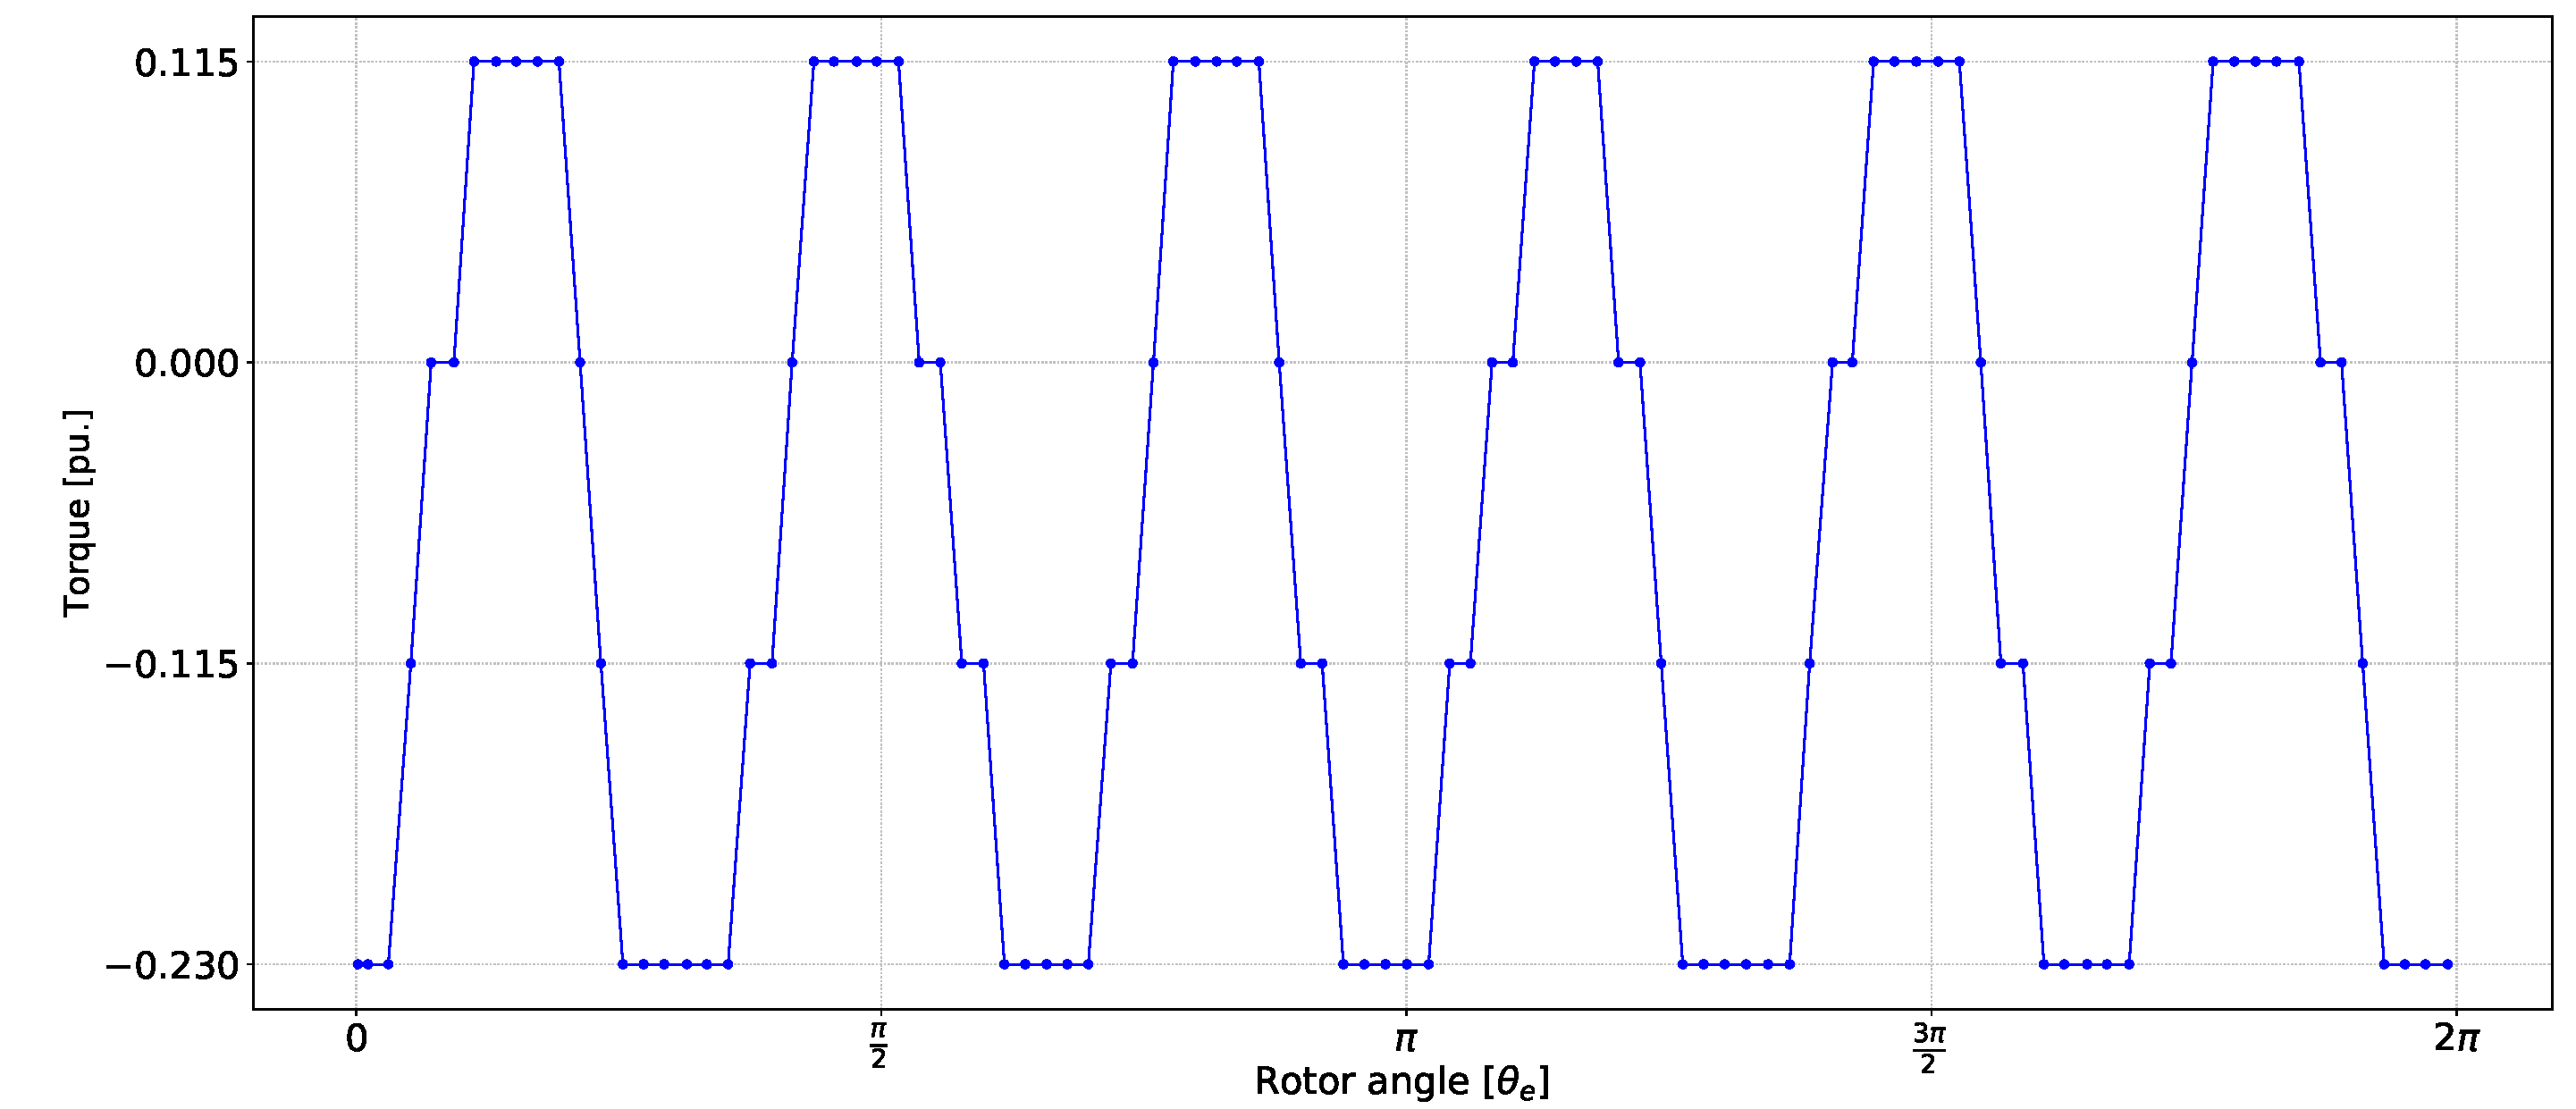
\includegraphics[width=\textwidth]{images/learned-compensation-pattern.pdf}
    \caption{\small Learned compensation pattern with respect to the rotor angle}
    \label{fig:learned_pattern_torque}
\end{figure}


\subsection{Q-learning algorithm}
Q-learning provides a capability for the agent to learn to act optimally in MDP \cite{RL:Watkins-Q}. The agent tries actions and evaluates the consequences in terms of received rewards and estimates of the next state value \cite{RL:Watkins-Q}. By repeatedly trying actions in all states, the agent eventually learns which actions are the best in overall \cite{RL:Watkins-Q}. The task of the agent is to determine an optimal policy that maximizes total discounted expected reward \cite{RL:Watkins-Q}. The discounted reward is calculated by repeatedly down-weighting recent rewards, by a factor of $\gamma \in [0, 1]$ \cite{RL:Sutton-Barto}
\begin{equation*}
    G_t = r_{t+1} + \gamma r_{t+2} + \gamma^2 r_{t+3} = \sum_{k=0}^{T} \gamma^k r_{t+k+1}
\end{equation*}
where $t$ is time step and $T$ is total number of steps and for continuous tasks, $T = \infty$. The number of down-weightings depends on the amount of steps taken and therefore the discounting makes historical rewards less valuable than rewards received recently. The discounting factor $\gamma$ makes it possible to adjust the discounting rate, which allows to control behaviour of the agent.

During learning, the agent observes the state $s_t$, selects and performs an action $a$, observes subsequent state $s_{t+1}$, receives a reward $r$ and adjusts its Q-values $Q(s_{t+1}, a_{t+1})$ using a learning factor $\alpha \in [0, 1]$. The update can be written as \cite{RL:Watkins-Q}
\begin{equation}
    Q(s_t, a_t) \leftarrow Q(s_t, a_t) + \alpha \cdot [r_t + \gamma \cdot \max_{a}Q(s_{t+1}, a) - Q(s_t, a_t)]
    \label{Eq:Q-learning}
\end{equation}
where $\max_{a}Q(s_{t+1}, a)$ corresponds action selection policy. In this case the agent selects the best action it perceives to be able to perform. The $\alpha$ is used to adjust how much weight single sequence gets in update, thus representing update step size. At early stages of learning, the agent policy is far from optimal, but the agent learns iteratively to pick better actions. The learning process can be stopped at any point and the Q-values can be saved for later use. After training, it is adequate to pick the best actions based on the learned and stored Q-values, $Q(s_{t}, a_{t})$.

During the learning phase, the agent must select and test actions in order to learn. The simplest action selection rule is to pick an action producing the highest estimated value, $\max_{a}Q(s_{t+1}, a)$. Such greedy action selection always exploits the current knowledge, which is problematic in case where better actions exist, but the agent is not aware of these. Better learning performance can be achieved by behaving greedily most of the time, but with small probability $\epsilon$, the agent may randomly test a new action. Action testing is called exploration. The methods allowing exploration with probability $\epsilon$ are called $\epsilon$-greedy methods. In noisy environments, these are better than plain greedy methods, as it requires more exploration to find the optimal actions due to noisier rewards. The measured speed signal with electric motors is often quite noisy, which advocates use of $\epsilon$-greedy action selection policy. \cite{RL:Sutton-Barto}

The probability $\epsilon$ is used to set balance between exploration and exploiting. The action selection policy can be described with \cite{RL:Sutton-Barto}
\begin{equation}
  a \leftarrow \begin{cases}
    \max_{a}Q(s_{t+1}, a),  & \text{with probability $1 - \epsilon$}.\\
    \text{a random action}, & \text{with probability $\epsilon$}.
  \end{cases}
  \label{Eq:epsilon-greedy}
\end{equation}
where $\epsilon$ can be a constant value or it can be also gradually decreased. By gradually decreasing $\epsilon$, the agent progressively relies more and more on learnt information. The probability $\epsilon$ is allowed to decrease to some small positive number, i.e., $0.01$, which ensures that agent does not completely stop exploring during training. The decay of $\epsilon$ can be implemented to happen with respect to training iterations
\begin{equation}
  \epsilon \leftarrow \begin{cases}
    k_\epsilon \,/\,(k_\epsilon + i), & \text{if $\epsilon > 0.01$}.\\
    0.01,        & \text{otherwise}.
  \end{cases}
  \label{Eq:glie}
\end{equation}
where the $k_\epsilon$ is some constant integer and $i$ is the iteration number. From \eqref{Eq:epsilon-greedy} and \eqref{Eq:glie} it can be seen that high $k_\epsilon$ value encourages the agent to explore more than with low $k_\epsilon$ value. By gradually decreasing the $\epsilon$, the learning may happen faster than with a constant value.


\subsection{Torque based learning scheme}
It has been discussed how the torque ripple problem can be formalized and how the agent learns through rewards, but it has been left unclear how the "goodness" of actions can be evaluated and what should be given as a reward. This ultimately depends on the objective and the system. In this study, the system is motor drive and the objective is to minimize torque pulsations. To meet the goal, the rewarding process should connect actions and torque pulsations. This connection allows the agent to perceive the influence of its actions, which makes it possible for the agent to adjust its behaviour in order to maximize the expected reward. A reward function can be used to generate a reward at each time instant.

Assuming that produced torque can be measured, the reward function can be very simple. The reward can be given based on how closely the agent is able to follow the desired torque value, $-|T^* - T_m|$. The expression is multiplied with $-1$ to make the agent to try to minimize the torque error. In order to maximize the reward and to minimize the error, the agent would need to find a way to compensate disturbances by using predefined actions.

The simple torque based learning scheme was tested in the simulator. The agent was trained to compensate for the sixth harmonic with only five different actions. The learning outcome can be seen in Fig. \ref{fig:learned_pattern_torque}. The rewards obtained by the agent during training were collected and the reward values are visualized in Fig. \ref{fig:qlr_torque_reward}. The reward plot shows that the agent clearly learns to reduce torque pulsations, since the periodical rewards reflecting torque error are getting better. It can be observed that learning gets continually slower as it gets constantly harder for the agent to find better ways to reduce pulsations. Majority of the improvement happens in the first few hundred iterations. It should be also noted that the agent is never able to fully compensate for pulsations with only five actions, hence the reward average will never reach zero. Another important observation from Fig. \ref{fig:qlr_torque_reward} is the amount of variance in rewards. Not all actions are successful which results to bad rewards. In this particular problem, one bad action can lead to sequence of bad rewards, since recovering takes time. Rewards can be seen to dip even after prolonged training. This implies that the most recent Q-values are not necessarily the best. Therefore, instead of saving the most recent Q-values, the best values should be selected for example using the reward average.
\begin{figure}[tb] 
    \centering
    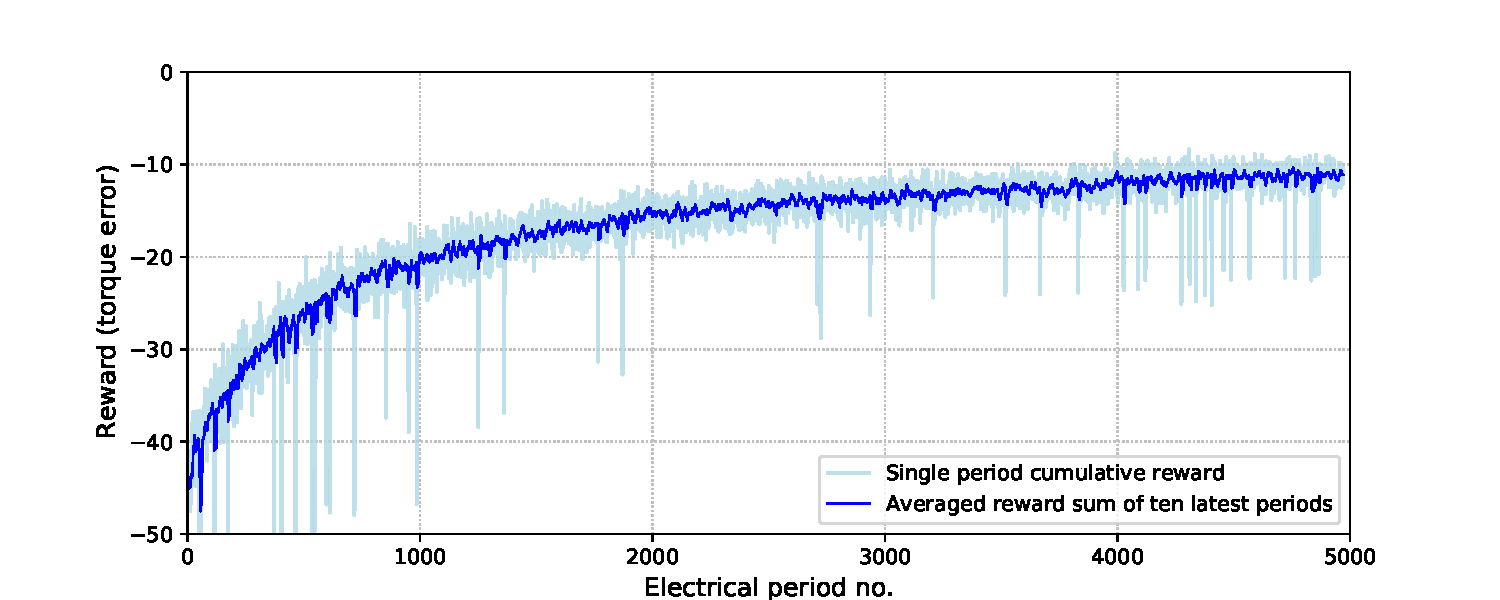
\includegraphics[width=\textwidth]{images/torque-reward-history.pdf}
    \caption{Rewards obtained during simulated training of the agent}
    \label{fig:qlr_torque_reward}
\end{figure}

The torque based learning scheme is unfortunately highly impractical, since torque measurement or suitable estimate is rarely available. Creating an accurate torque estimator is a complex task and therefore this option should be avoided. It is also good to be aware that already existing torque estimation scheme cannot be utilized. The agent produces torque by injecting to q-axis current reference $i^*_q$ which corrupts the torque signal for learning purposes. If the agent sees its own injections directly from the estimated torque signal, then often the best method to minimize the pulsations is to do nothing.


\subsection{Speed based learning scheme}
The learning can be done by utilizing the speed signal. A speed based compensation scheme is more practical compared to the torque based counterpart, since speed sensors are more commonly available by default than torque measuring instruments. Furthermore, by inspecting the ILC compensator development trend in \cite{ILC:2004} and \cite{ILC:2005}, it appears that the speed signal based compensator was found more successful.

The motor speed depends on torque according to \eqref{Eq:transfer_function}. By inspecting computed speed and torque in Fig. \ref{SDM_speed_torque}, it can be observed that there is a phase shift between the two signals. This is exceedingly problematic when considering speed based rewarding. If the effects of torque alternation are not immediately visible, then the agent cannot know what consequences its actions had. In the worst case, the agent tries to apply brief torque impulses that are invisible for it, but stress the system in reality. Therefore, the prior rewarding scheme cannot be used directly with speed based learning. The reward function must be modified.

The occurring delay between torque and speed pulsations \eqref{Eq:transfer_function}, must be accounted when giving reward. With neural networks, such problems requiring memory could be solved by using recurrent networks \cite{RL:memory}. These feed the output signal back into the network, thus allowing the system to memorize events. This would solve the delay related rewarding problem. Unfortunately, these methods cannot be used directly with the tabular representation that the Q-learning uses. Nonetheless, the idea of saving and reusing the data on subsequent iterations can be utilized. The previous observations can be stored into memory and these can be used in determining reward with the current observations. 

It was found best approach to use only the previous and current observations to give reward. Greater amount of rewards attenuate the weight of the previous and current observations, which are the most important ones. The reward function used in the experiments is given by
\begin{equation}
    r_t = -(|\omega^{*}_{m, t} - \omega_{m, t}| + \lambda \cdot |\omega_{m, t} - \omega_{m, t-1}|)
    \label{Eq:reward-function}
\end{equation}
where $\omega^{*}_{m, t}$ is the speed reference at time instant $t$ and $\lambda$ is a weighting factor. The reward function encourages the agent to select such actions that allow following of the speed reference and the speed should change as little as possible between steps. It was found that indirect learning from the speed signal takes more time than directly using torque values for giving reward.

The agent was found to behave differently depending on how the reward terms are weighted with parameter $\lambda$. Simulation results in Fig. \ref{fig:lambda} show effects of different $\lambda$ weights. It can be observed that speed pulsations become smaller when $\lambda$ is increased up to value $32$. After going past $32$, the pulsations appear to grow again, possibly because the agent gets punished so little from not staying in the reference.
\begin{figure}[htb] 
    \centering
    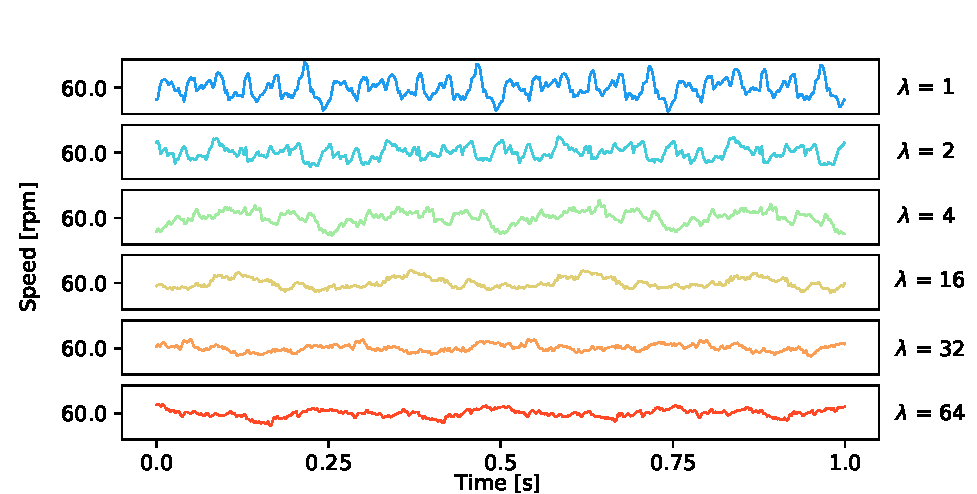
\includegraphics[width=\textwidth]{images/lambda_multiplier.pdf}
    \caption{Simulated effects of different $\lambda$ weights}
    \label{fig:lambda}
\end{figure}


\subsection{Hyperparameters} \label{hyperparameters}
Hyperparameters are parameters that are set before training and have an effect on the learning rate and outcome. Such parameters are the discount factor $\gamma$, learning rate $\alpha$, weighing factor $\lambda$ and coefficient $k_\epsilon$ used to set epsilon decay rate. These parameters must be set only once for a particular system. The same hyperparameters are likely to work with variety of different PM motors as long as the whole system stays similar. In \cite{RL:atari} the same hyperparameters were successfully used to train the agent to play various video games. In simulations, the same hyperparameters were successfully used to train the compensator to work with all four tested PM motors. By using the same hyperparameters, the training process may not be optimal, but this approach can still yield satisfying learning results.

Figures \ref{fig:gamma}, \ref{fig:alpha} and \ref{fig:glie} show averaged cumulative sums of rewards obtained during one mechanical revolution. Averaging makes the trends more clear, since instaneous rewards can be very noisy. Nevertheless, the most important information that the plots provide are the relative growth rates between the different scenarios and this information can be used for concluding approximately the best hyperparameter values for the system. In general, such hyperparameter values should be selected that provide the best learning outcome and make the learning happen in the shortest time. When considering the learning rate, the first few hundred iterations should be emphasized if the agent can cause superfluous stress to the system. Periodical rewards in Fig. \ref{fig:qlr_torque_reward} illustrate that most of nonsensical actions are performed during early phase of training. Therefore, the risk of damaging the system is the greatest when training is started. Since unnecessarily large current injections generate heat, it is desired to select such hyperparameter values that let the agent to reach sufficient performance level quickly, even at the expense of slightly decreasing total learning rate.
\begin{figure}[htb] 
    \centering
    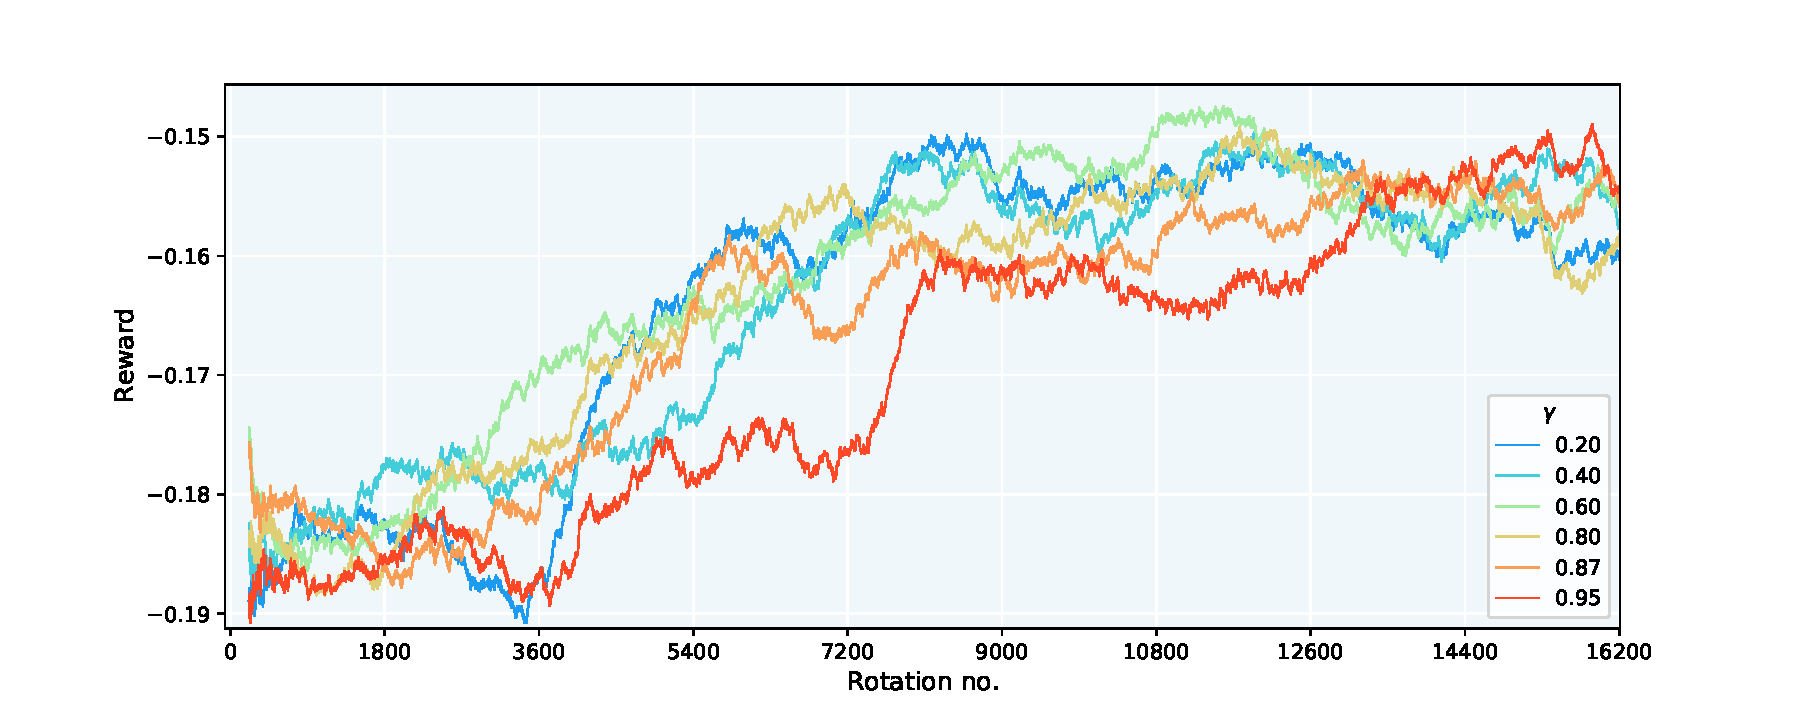
\includegraphics[width=\textwidth]{images/Qgamma_wide.pdf}
    \caption{\small Learning simulated with different $\gamma$ values}
    \label{fig:gamma}
\end{figure}

The parameter $\gamma$ defines discount rate for rewarding. It has effect on how the agent perceives rewards and how shortsighted its actions are. Figure \ref{fig:gamma} shows that early learning takes longer with high $\gamma$ values. With more moderate values the agent starts to learn more quickly, thus making less completely nonsensical actions. The parameter $\gamma = 0.6$ was selected to be used in simulations and experiments, as it appears to make the early learning quick and stable.
\begin{figure}[htb] 
    \centering
    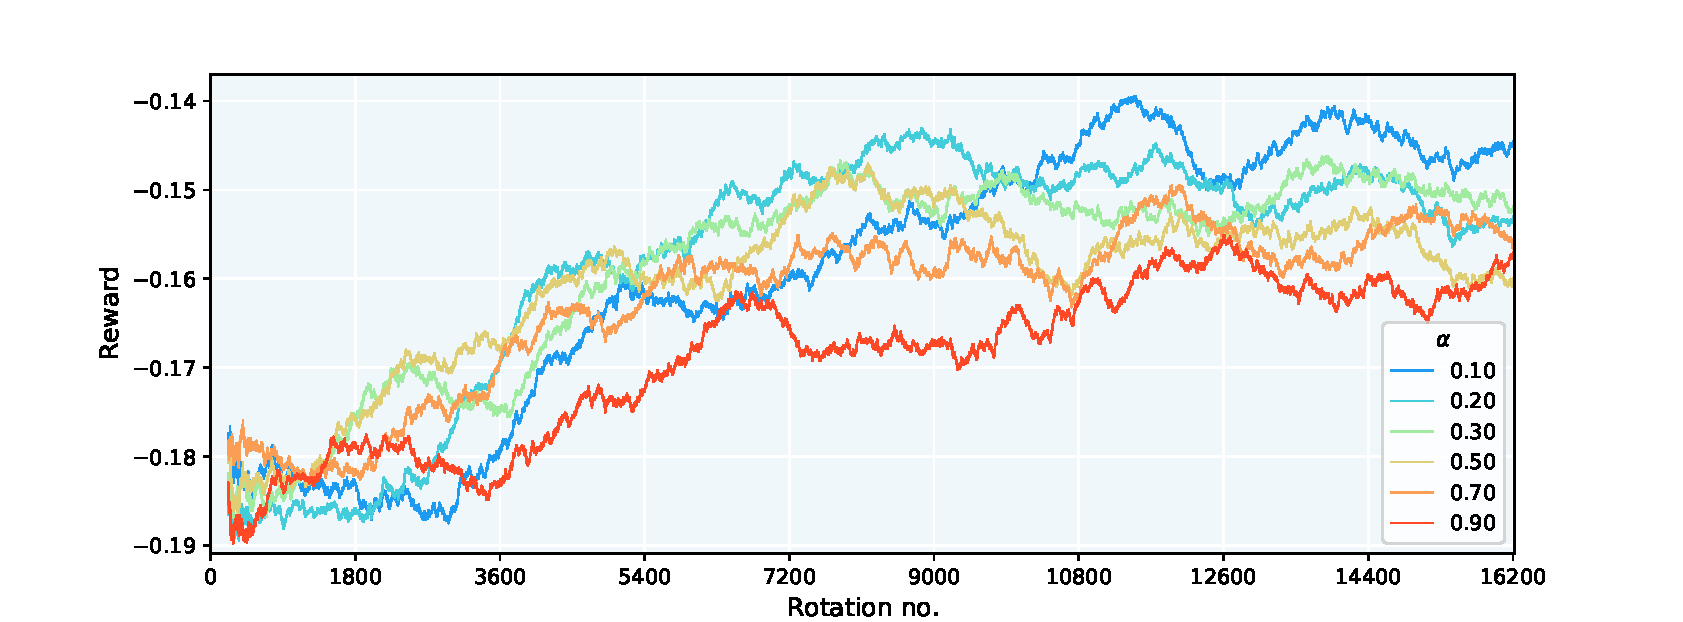
\includegraphics[width=\textwidth]{images/Qalpha_wide.pdf}
    \caption{\small Learning simulated with different $\alpha$ values}
    \label{fig:alpha}
\end{figure}

In order to demonstrate the effects of the learning rate $\alpha$ in the simulation environment, noise had to be generated. Therefore, white noise having maximum amplitude of 30\% of the measured speed, was injected to the compensator speed input signal. With constant $60$ rpm speed, the compensator speed input can vary between $42-78$ rpm due to added noise. Figure \ref{fig:alpha} shows that learning is slower, when doing considerable updates with large $\alpha$. With smaller update steps, the learning is faster in noisy environment. While considering the early learning speed, the value of $\alpha = 0.3$ was selected to be used.

The $\epsilon$-greedy policy is used for training. The different $\epsilon$ decrease rates lead to different learning behaviour. Figure \ref{fig:glie} illustrates learning with different $k_\epsilon$ values. It appears that there is no significant differences between selections. Value of $k_\epsilon = 300$ was selected to be used in simulations.

\begin{figure}[htb] 
    \centering
    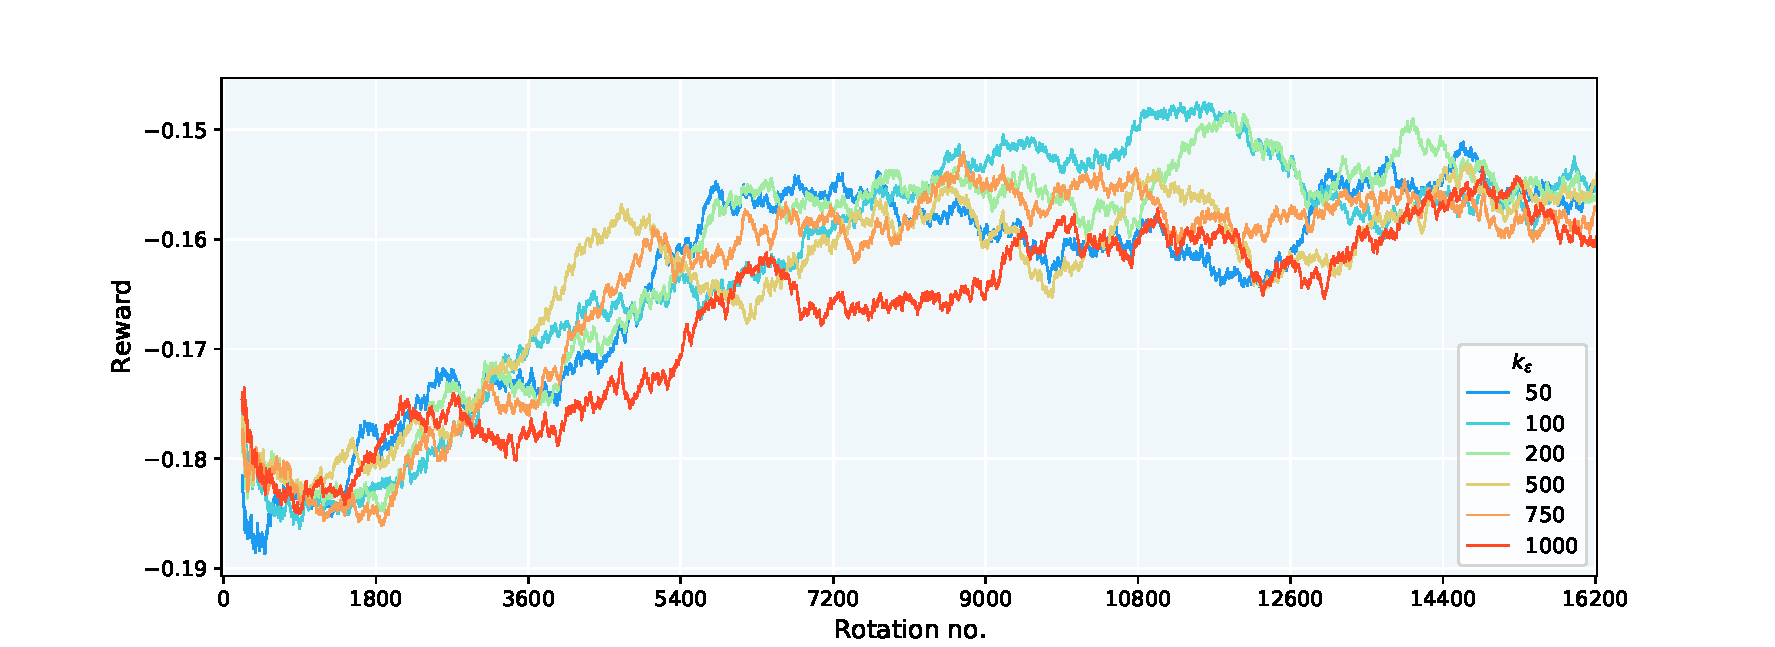
\includegraphics[width=\textwidth]{images/Qk_wide.pdf}
    \caption{\small Learning simulated with different $k_{\epsilon}$ values}
    \label{fig:glie}
\end{figure}

\clearpage
